% !TeX spellcheck = en_US
% !TeX encoding = UTF-8
%\documentclass[a4paper,headsepline,12pt,bibliography=totoc]{scrreprt}
\documentclass[a4paper,headsepline,12pt]{scrartcl}
\usepackage[T1]{fontenc}
\usepackage[utf8]{inputenc}
\usepackage[english]{babel}
\usepackage[hyphens,spaces,obeyspaces]{url}
\usepackage[pdfborder={0 0 0}]{hyperref}
\usepackage[backend=bibtex,style=numeric-comp]{biblatex}
\usepackage[babel,style=english,english=american]{csquotes}
%\usepackage[singlespacing]{setspace}
\usepackage{lmodern}
\usepackage[usenames,dvipsnames,table]{xcolor}
%\usepackage{cite}
\usepackage[binary-units]{siunitx}
\usepackage{float}
\usepackage{setspace}
\usepackage{mathcomp}
\usepackage{amsmath}
\usepackage[font=small]{caption} 
\usepackage[font=footnotesize]{subcaption}
%\usepackage{ae}
\usepackage{caption}
\usepackage[final]{graphicx}
\usepackage{listings}
\usepackage{enumitem}
\usepackage{adjustbox}
\usepackage{tikz}
\usetikzlibrary{mindmap}
\usepackage{xspace}
\usepackage{amssymb}
%\usepackage{showframe}
%\usepackage[prependcaption,textsize=tiny,colorinlistoftodos]{todonotes}
\usepackage[disable]{todonotes}

\lstset{
	%numbers=left,
	breaklines=true,
	tabsize=4,
	basicstyle=\ttfamily,
	commentstyle=\color{red},
}

% alle floats zentrieren
\makeatletter
\g@addto@macro\@floatboxreset\centering
\makeatother

\newcommand{\eg}{e.\,g.\xspace}


\title{AIR - Homework 5}
\date{\today}
\author{Maximilian Mensing\\Torsten Jandt}


\begin{document}
\maketitle{}
\section{Informed Search Strategies}
\begin{adjustbox}{totalheight=16cm}
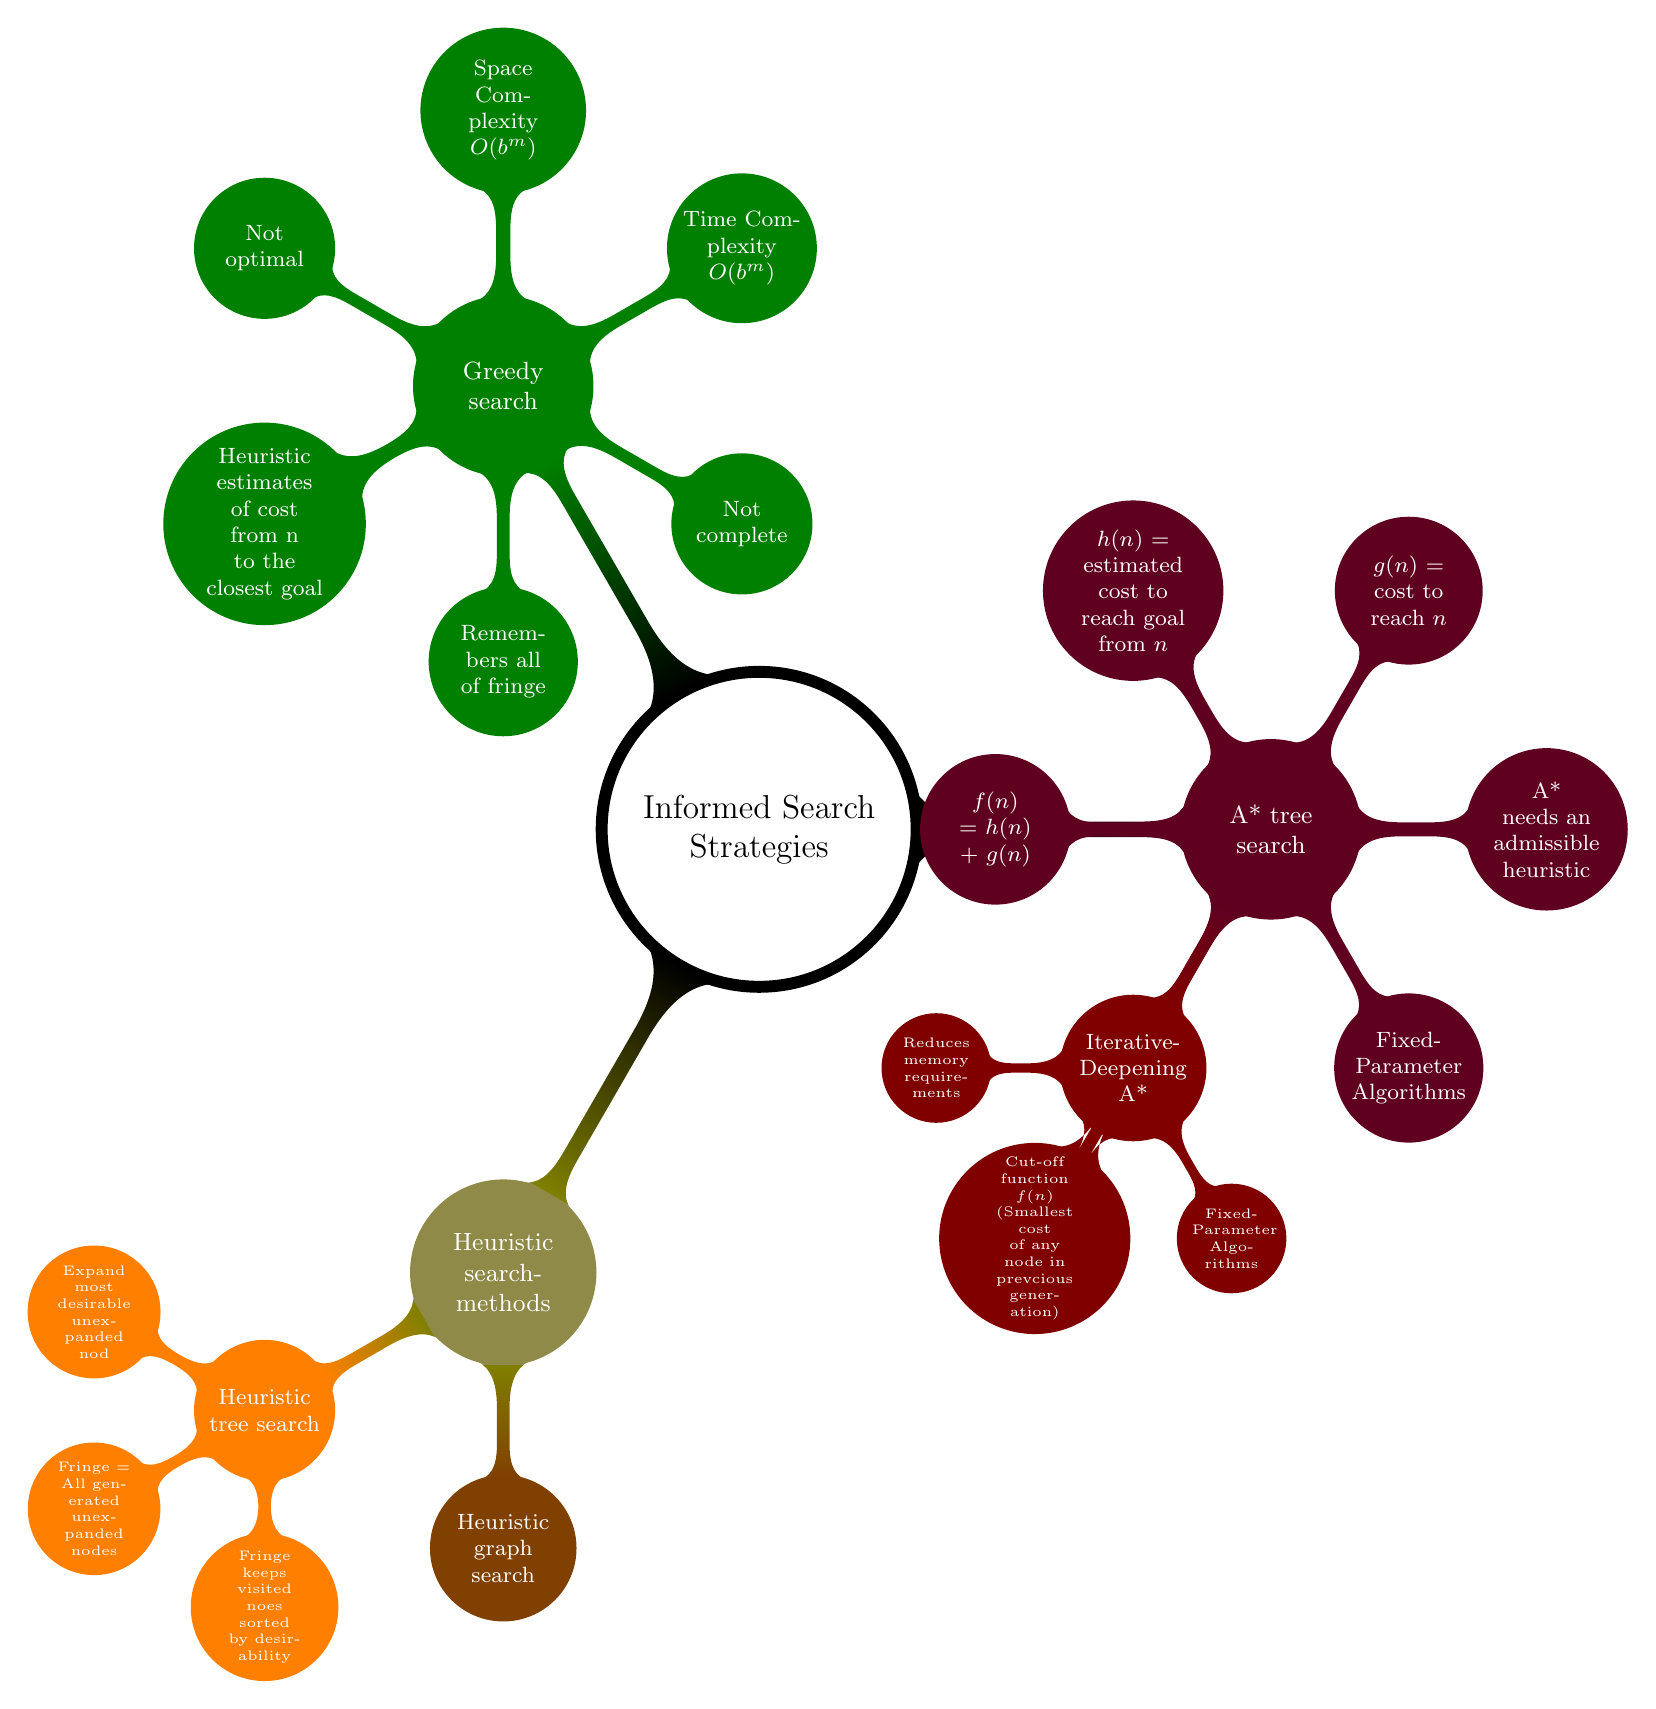
\begin{tikzpicture}[
  mindmap,
  every node/.style={concept, execute at begin node=\hskip0pt},
  root concept/.append style={
    concept color=black, fill=white, line width=1ex, text=black
  },
  text=white, grow cyclic,
  level 1/.append style={level distance=6.5cm,sibling angle=120},
  level 2/.append style={level distance=3.5cm,sibling angle=60},
  level 3/.append style={level distance=2.5cm,sibling angle=60}
]

\node[root concept] {Informed Search Strategies} % root
child[concept color=yellow!50!black] { node  {Heuristic searchmethods}
	child[concept color=orange] { node {Heuristic tree search}
		child { node {Expand most desirable unexpanded nod} }
		child { node {Fringe = All generated unexpanded nodes} }
		child { node {Fringe keeps visited noes sorted by desirability} }
	}
	child[concept color=orange!50!black] { node {Heuristic graph search}
	}
}
child[concept color=purple!50!black] { node {A* tree search}
	child { node {Complete} }
	child { node {Worst case: \(O(state space)\)} }
	child { node { Best case: \(O(d)\)}}
	child { node {Fixed-Parameter Algorithms} }
	child { node {A* needs an admissible heuristic}}
	child { node {\(g(n)\) = cost to reach \(n\)} }
	child { node {\(h(n)\) = estimated cost to reach goal from \(n\)} }
	child { node {\(f(n)\) = \(h(n)\) + \(g(n)\)} }
	child[concept color=red!50!black] { node {Iterative-Deepening A* }
		child { node {Reduces memory requirements} }
		child { node {Cut-off function \(f(n)\) (Smallest cost of any node in prevcious generation)} }
		child { node {Fixed-Parameter Algorithms} }
	}
}
child[concept color=green!50!black] { node {Greedy search}
child { node {Not complete} }
child { node {Time Complexity \(O(b^m)\)} }
child { node {Space Complexity \(O(b^m)\)} }
child { node {Not optimal} }
child { node {Heuristic estimates of cost from n to the closest goal} }
child { node {Remembers all of fringe} }};
\end{tikzpicture}
\end{adjustbox}
\newpage
\section{IDA vs DFS}
In state spaces with a very high number of states in every layer DFS ( and thus a high branching factor) performs better than IDA
\section{Informed Search Strategies Evaluation}

\begin{table} [ht!]                                             
\centering                                                
\begin{tabular}{|c|c|c|c|c|c|c|c|c|}    

\multicolumn{4}{c}{ \textbf{Performance of IDA on three maps}}   \\                                           
\cline{1-4}                                                    
\multicolumn{1}{|c|}{} & MAP1 & MAP2 & MAP3  \\
\hline                                                    
Deepest level reached & 511 & 255 & 1143  \\ 
\hline                                                         
Total of stored nodes & 7363 & 6999 & 35410 \\
\hline                                                         
Total of visited nodes & 22433 & 21943 & 116461 \\ 
\hline
                                                 
\end{tabular}                                             
\caption{}                                  
\label{table:maps}                                
\end{table}  
Table \ref{table:maps} shows that the amount of visited and stored nodes strongly depends on the maps size. While searching the state space for solution, a greater state space has to be traversed. The deepest level reached stands for the state distance between to goals.  On the second map the goals are almost sorted, resulting in less states to be visited when searching for the next goal.




\end{document}